\documentclass{article}
\usepackage{tikz,pgfplots}
%\pgfplotsset{colormap={name}{
%	color(0cm)=(blue);
%	color(1cm)=(green);
%	color(2cm)=(yellow)
%	color(3cm)=(red)}}
\pgfplotsset{colormap={blues}{
       color(0cm)=(white);
       color(1cm)=(blue)}}

\definecolor{diplom1}{rgb}{0.0 0.4 1.0}
\definecolor{diplom2}{rgb}{0.0 0.0 0.6}
\definecolor{diplom3}{RGB}{153,0,0} %unirot
\definecolor{diplom4}{RGB}{232,215,23}
\definecolor{diplom5}{RGB}{51,37,60}

\definecolor{unirot}{RGB}{153,0,0}
\definecolor{unirot_hell}{RGB}{255,228,225}
\definecolor{lightblue}{RGB}{242.2,249.88,255}

\begin{document}

% \begin{tikzpicture}[
%          scale=1.0,>=stealth,domain=-4:4,samples=100,
%          declare function={
%          q = 0.1;
%          distrib(\x) = cos(\x);
%        }]
%  \draw[->,thick] (-0.2,0) -- (10.2,0) node[right] {$E$};
%  \draw[->,thick] (0,-0.2) -- (0,6.2) node[anchor=north east] {$\left. \frac{\mathrm{d}}{\mathrm{d}t}
%                                                   |f_{fi}|^2 \right|_{t=0}$};
%  \draw [color=black,domain=-4:4,smooth,very thick]    plot
%         (\x,{distrib(\x)});% node [anchor=south] {Cauchy distribution};
% \end{tikzpicture}

 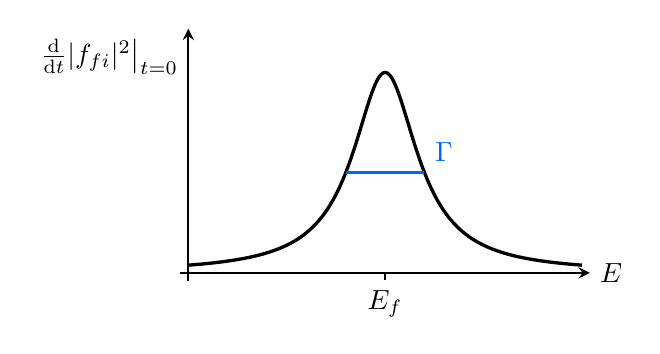
\begin{tikzpicture}[
          scale=0.5,>=stealth,domain=0.5:10,samples=100,
          declare function={
          gamma = 1.0;
          factor = 16.0;
          halfmax = factor * 0.15915;
          x_0 = 5.0;
          distrib(\x) = factor/3.14159 * gamma / ((\x-x_0)^2 + gamma^2);
        }]
%     \tiny
%  \draw[very thin,color=gray] (-0.1,-0.1) grid (4.9,4.9);
  \draw[->,thick] (-0.2,0) -- (10.2,0) node[right] {$E$};
  \draw[->,thick] (0,-0.2) -- (0,6.2) node[anchor=north east] {$\left. \frac{\mathrm{d}}{\mathrm{d}t}
                                                   |f_{fi}|^2 \right|_{t=0}$};
  % add ticks
  \draw [thick] (5,0) -- (5,-5pt) node [anchor=north] {$E_f$};

  \draw [color=black,domain=0:10,smooth,very thick]    plot
         (\x,{distrib(\x)});% node [anchor=south] {Cauchy distribution};
  \draw [-,very thick,diplom1] (4.0,halfmax) -- (6,halfmax)
         node [anchor=south west] {$\Gamma$};
 \end{tikzpicture}

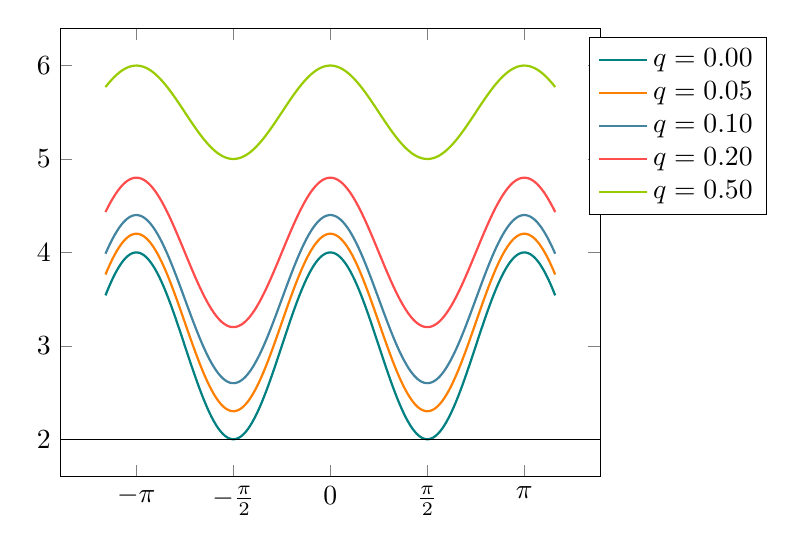
\begin{tikzpicture}
    \begin{axis}[domain=-0.5-pi:0.5+pi,
                 samples = 200,
                 xtick={-3.14159,-1.57089,...,3.14159},
                 xticklabels={$-\pi$,$-\frac \pi 2$,0,$\frac \pi 2$,$\pi$},
                 cycle list name = exotic,
                 legend style={anchor= north west}
                 ]
    \foreach \q in {0.00,0.05,0.10,0.20,0.50}{
      \addplot+[mark = none,
               thick
               ]
               {4*\q + 2 + 2*cos(deg(x))^2 + 2*\q*sin(deg(x))^2}; 
      \addlegendentryexpanded{$q=\q$}
               }
      \draw[] (axis cs:\pgfkeysvalueof{/pgfplots/xmin},2) -- (axis cs:\pgfkeysvalueof{/pgfplots/xmax},2);
    \end{axis}
\end{tikzpicture}



	\end{document}
